\chapter{Bewertung und Zusammenfassung}
\label{chapter:evaluation}

\section{Methodik und Ergebnisse}
\emph{Design-Thinking} (Kap. \ref{def-design-thinking}) hat als Methode die vorliegende Arbeit erheblich geprägt. Anfänglich wurde sie beiläufig berücksichtigt und gewann für die Erforschung der Ursachen erheblich an Bedeutung. Der Prozess ist hierbei kein fester Rahmen, sodass Elemente aus \enquote{Requirement-Engineering} und ein agiler Vorgang eine Rolle gespielt haben. Vielleicht ist das gerade die Stärke, weil der Prozess Offenheit vorsieht und individualisiert werden kann. Wichtig ist der Anfang des Prozesses mit \emph{empathize}.
\medskip
\\
Dieses Modell ist auch von Agilität und Kontinuität geprägt, worin sich das Ergebnis ständig verbessert. Mittendrinn können auch Iterationen erfolgen.
Besonders effektiv ist es, wenn dabei aus dem aktuellen Zustand heraus ein Perspektivwechsel gezielt hin zur Problemquelle stattfindet. Am Ende kann mit einer erheblich größeren Datenmenge eine Synthese aus allen Perspektiven generiert werden als Deduktion. Dabei war die Ausgangssituation von einem sehr eingeschränkten Problembild geprägt. Eine Immersion (Kap. \ref{def-design-thinking}) hat das Horizont innovativ und effektiv erweitert. 
Der Design-Thinking Prozess könnte als ein \enquote{Quick-Search} für Innovation gesehen werden. Daneben sind andere Gestaltungsmethoden ebenfalls zu betrachtet.
\medskip
\\
Sie hinterlässt jedoch viele Artefakte\footnote{Anhang: Docker Images für Jenkins Agenten\label{appendix:docker}} und es Besteht die Gefahr zu divergieren, da sie mit einer erheblichen Geschwindigkeit induktiv vorgeht und auf kontinuierliche Verbesserung der Prototypen beruht. Dadurch entstehen viele Artefakte.
Für die Qualitätssicherung der Lösung verlangt es einen effizienten Vorgang der Integration der Komponenten und Implementierung einer Lösung mit entsprechenden Methoden. Für eine erste Lösungsrichtung bieten ihre Syntheseschritte durch ständige Iterationen eine schnelle Deduktion. Ergebnisse können entsprechend von einer Innovationsphase in die Entwicklungsphase übergehen, in welchem die Qualitätssicherung in einer separaten Umgebung sichergestellt wird. Agilität ist daher immer mit einer Nutzen-Risiko Analyse verbunden.

\subsection{Aus CI/CD zu einer nachhaltigen IT}
Die Anfangssituation aus der \ac{SEU} in Kap. \ref{grundlagen:ci-in-banken} wurde bis zu einer unzumutbaren Hindernissschwelle bearbeitet und erste Lösungsansätze mit gängigen Standards beschrieben. Die vorgeschlagenen Ansätze lösen jedoch nicht den Ursprung des Problems, da sie umfassende Auswirkungen und Anpassungen nach sich ziehen, die eine Transformation der ganzen Organisation fordern. 

Für die Ursache des Problems fand ein Wechsel der Perspektive in Kap. \ref{section:Goldman} zu einem Wettbewerber statt, der eine Transformation bereits durchgemacht hat. Diese Transformation ist als Fallbeispiel von \citet{Gupta:2017} empirisch beschrieben und enthält wiederum verschiedene Stellungnahmen aus der Managementebene.

In den Schritten \emph{empathize}, \emph{define} und \emph{ideate} wird die Ursache des Problems analysiert möglichst ohne vorherige Annahme zur Quelle des Problems. Wichtig ist, dass hierbei wirklich die Perspektive gewechselt wird und eine Immersion in die Umgebung des Kunden stattfindet. Daher kann diese Gruppe statt Analyse \cite{yüksel:digit} auch Immersion genannt werden. 

Hierbei wurde in dieser Arbeit die Erfolge der betrachteten Perspektive hervorgehoben und untersucht. Anschließend wurde eine Steigerung dieses Erfolges gesucht.
\medskip
\\
Hierfür sind Schritte in \emph{Synthese} eine Datenerhebung \cite[S. 61]{yüksel:digit} durch Gestaltung von Zukunftszuständen, die nach \citet[S. 14]{Alt2017} für eine \emph{Vorwegnahme künftiger Innovationen} von besonderer Bedeutung ist. 

Die Opportunitäten durch Goldman Sachs Plattform \cite{Gupta:2017} und der Hintergrund von disruptiven Technologien \cite{Fernandez:2020} wurde zum Anlass genommen Ideen zu formulieren. In Kap. \ref{section:Goldman} wurden weitere Zukunftszustände gestaltet.
Wichtig ist hierbei, dass ungezwungen so viele Daten wie möglich generiert und erhoben werden. Mit dem richtigen Verständnis aus den vorigen immersiven Schritten kann eine Deduktion nach den Anforderungen des Kunden stattfinden. 

Die vorgeschlagenen Ideen werden daher mit einer anderen Perspektive weiter gefiltert. Im Rahmen des Finanzwesens standen den disruptiven Technologien und FinTechs auf dem ersten Blick die Regulatorik entgegen.

Die erhobenen Daten waren anfänglich neue Technologien zur Lösung des Problems und Einschränkungen im Rahmen der IT-Architektur und Regulatorik. Die regulatorischen Forderungen an sich sind keine Einschränkung gegenüber Innovationsverläufen. Die Einschränkungen werden durch die Symptome der diskontinuierlichen Legacy-IT hervorgerufen, da Transformationen nicht durch immaterielle Zustände beschränkt werden können.

Das Problem hierbei ist, dass ab einer gewissen Größe des Unternehmens sie sich gegenseitig voraussetzen. Die Optimierung der Überwachungs- und Steuerungsprozesse erfordert eine agile Architektur, die widerum durch sich selbst eingeschränkt ist. \citet{Ganswindt2006} benennt das Ganze als Henne-Ei Problem, dass an vielen Stellen in unterschiedlichen Formen auftaucht.
\medskip
\\
Daher wurde früh erkannt, dass die Ursache in der Transformationsfähigkeit der Organisation liegen könnte. Aus einer gemeinsamen Betrachtung der Sicht der \ac{SEU} \ref{grundlagen:ci-in-banken} und Goldman Sachs \cite{Gupta:2017} spielten hierfür neben regulatorischen Anforderungen als Einschränkung auch die Kultur als Antrieb eine wichtige Rolle.

Der Perspektivwechsel mit der \emph{Design-Thinking} Methode \ref{def-design-thinking} durch eine Iterationen in den anfänglichen Empathize Zustand ermöglichte die Sicht der Regulatorik auf Technologien und Veränderungen zu betrachten und ist daher für die Generierung von weiteren Ergebnissen wichtig, bis die Lösung der Problemursache gefunden wurde.

Die Aufsicht wäre sicherlich nicht daran interessiert noch mehr Komplexität durch zu präzise Anforderungen zu manifestieren. Die Ermessensfreiheit der Institute setzte Gestaltungsfähigkeit voraus.
\medskip
\\
Hierfür wurden Prototypen nach \emph{Design-Thinking} gestaltet, die unweigerlich zeigen, dass antreibende Anlagen zur Innovationsförderung wichtig sind. Für die Priorisierung fehlte dabei ein klares Steuerungsprozess, daher wurde das Modell mit den dargestellten Ergebnissen kontinuierlich verbessert.


\paragraph{Prototyp: Regelung der Transformation}
Für Prozesse wird im Rahmen des Innovationsdrucks vom IT-Management gerne auf Frameworks zurückgegriffen, wie zum Beispiel ITIL (Kap. \ref{def:itil}), worin Services sich bezüglich ihres Innovationsbeitrags messen lassen sollen \cite{Alt2017}. Im Rahmen dieser Arbeit wurden die Frameworks wie ITIL oder auch das offene Framework IT4IT wahrgenommen, jedoch bewusst nicht weiter untersucht. Im Rückblick kann festgestellt werden, dass viel mehr ein klares Bild vonnöten ist, was Frameworks wie ITIL bezwecken sollen, vor allem für das \ac{ITM}.
\medskip
\\
Es kann festgestellt werden, dass die Darstellung in (Abb. \ref{fig:digit-trans}) einen Beitrag für das Verständnis für Innovationskraft eines IT-Produktes leistet, um wiederum für eine IT-Strategie mit klaren Metriken zu priorisieren. Daraus wird klar, dass antreibende Technologien eine Anlage für die Generierung weiterer Innovationen sind. Die antreibenden Faktoren, die aus dem Ziel der Maximierung der Transformationsbewegung generiert wurden stellen möglicherweise eine Anforderung für Antriebe oder antreibenden Anlagen dar. Hieraus könnten weitere Ansätze generiert werden, um gezielt die Effektivität einer Innovation zu messen. Diese wäre wichtig für eine Priorisierung seitens \ac{ITM}.

Das schwierige ist jedoch hierbei die Transformation zu steuern und somit die Bewegungen zu kontrollieren. Das Finanzwesen erfordert eine Organisation mit absehbaren Manövern. Starke Bewegungen in Form von disruptiven Sequenzen sind riskant. Daher wird eine Transformation in Zusammenhang mit Disruptivität als Gefahr gesehen \cite{eba:2019}.

Aus diesem Hintergrund wurde ein weiteres Modell erzeugt mit Kontinuitätskonzept und einer Anhäufung von antreibenden Anlagen, wodurch einerseits disruptive Sequenzen linearisiert werden und gleichzeitig ein kontinuierlicher Antrieb entsteht, so die Theorie.

\section{Ökologisches Veränderungsmodell der IT}
\begin{figure}[htbp]
 \centering
 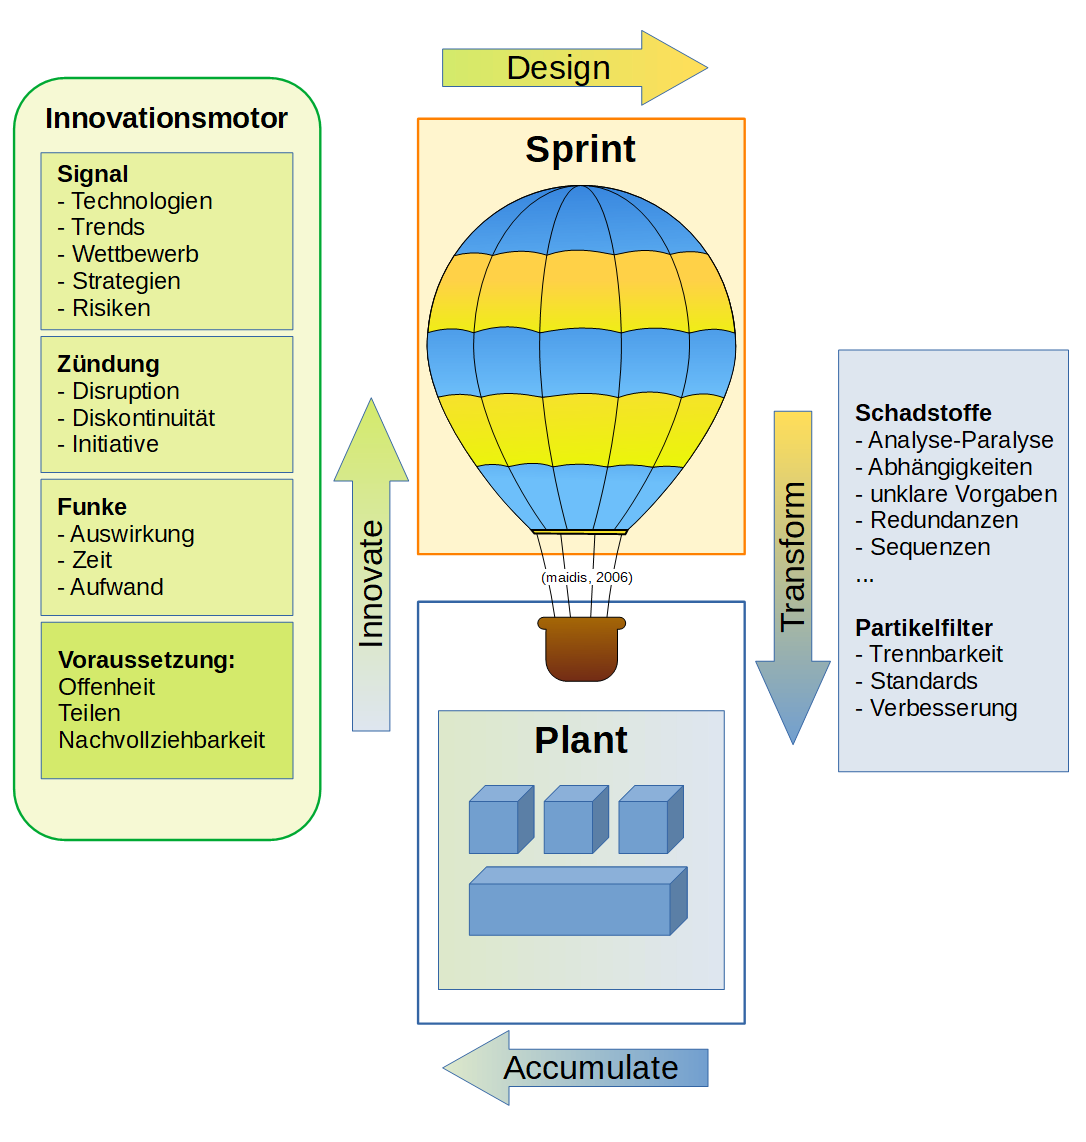
\includegraphics[width=1.0\textwidth]{gfx/digital-transformation-lifecycle-by-selim4.PNG}
 \caption{Ökologisches Veränderungsmodell der IT: IDTA-Modell, eine Erweiterung von Innovate-Design-Transform \cite{Koch2016} mit Anhäufung von Innovation \cite{Ganswindt2006} (Quelle: eigene Darstellung, Heißluftballon von \citet{maidis_2006})\label{fig:digit-trans-idt}
 } vgl. (Kap. \ref{idta-modell-chap})
 \end{figure}

Die Darstellung in (Abb. \ref{fig:digit-trans-idt}) ist eine Vorwegnahme eines künftigen Zukunftzustandes nach \cite{Alt2017}, die aus einer Orientierung nach \emph{Design-Thinking} Schritten entstanden ist und ständigen Iterationen ausgesetzt war, die den Rahmen dieser Arbeit sprengen würden. Nach der Identifizierung von möglichen Antrieben der Transformation, wurde \cite{Ganswindt2006} genauer untersucht. Nach dem Fund des \emph{Treibstoffs}\footnote{Begriff aus \cite{Ganswindt2006}}  musste ein Motor her. Die Regelung der Transformation durch manuelle, sequenzielle Abläufe erzeugt durch ihre Ineffizienz viele Schadstoffe die sich als einschränkende Faktoren materialisieren. Die Anhäufung dieser Faktoren ist das Ergebnis in Form einer Legacy- und Schatten-IT.

Für eine nachhaltige Organisation gehört es sich ihre Schadstoffe mit dem Einpflanzen von antreibenden Anlagen zu reinigen.

\section{Zusammenfassung und Ausblick}
Es ergibt sich ein Gesamtbild, dass die aufgeführten Faktoren der Veränderungsprozesse keine direkte Ablauf- oder Handlungsanweisungen darstellen. Daher kann das Problem der Priorisierung in der IT-Strategie stammen.

Diese leiten sich aus dem gegenwärtigen Zustand ab und beschreiben \emph{Einflüsse} gegen Veränderungsprozesse und haben wesentliche Auswirkungen auf ihren Ablauf. Insbesondere die antreibenden Faktoren für Veränderungsprozesse können als ihre funktionalen Anforderungen gesehen werden.

Das IT-Risikomanagement sieht mit ihren Maßnahmen jedoch in Disruptionen die Gefahr. \citet{Fernandez:2020} unterscheiden dabei Disruption und Diskontinuität. Etablierte Organisationen sind gegenüber Disruption Handlungsunfähig. Dabei geht die eigentliche Gefahr aus der Manifestierung von Diskontinuitäten aus. Diskontinuierliche Technologien weisen einen erheblich höheren Widerstand gegenüber der dominanten Technologie auf \cite{Fernandez:2020}. 

Die Diskontinuität ihrer Legacy-IT hat das Finanzwesen als Geisel genommen und das IT-Risikomanagement zu ihrem Helfer gemacht.

Kontinuierliche Ansätze wie \emph{DevOps} und \emph{Design-Thinking} helfen dabei die Veränderungsprozesse selbst agil und kontinuierlich zu gestalten und zu verstehen. Daher hat das IT-Risikomanagement sich nach Innovationsprozessen zu richten, um sich entgegen der Legacy-IT zu bewegen.
\medskip
\\
Darüber hinaus wird deutlich, dass die Informatik weitreichende Kompetenzen verfügt aus dem Zusammenhang heraus Probleme auch aus anderen Bereichen zu lösen. Beginnend von der Ausgangssituation eines vorwiegend technischen Problems haben innovationsorientiere Ansätze weitreichende Implikationen auf ihre nicht-technische Umgebung. Die Abkürzung IT sollte im Sinne einer Organisation künftig nicht für Informationstechnologie stehen sondern für \enquote{Innovation und Transformation}, wodurch es Bezug auf die Eingangs- und Ausgangsströme des Paradigmas \enquote{Innovate-Design-Transform} nimmt. Dazwischen liegt unser Ergebnis, das Akkumulieren als Wertschöpfung.
\medskip
\\
Kreative Methoden sind durch die ad-hoc Generierung von Prototypen oder Beschreibungen wichtige Mittel für die Gestaltung von immateriellen Zuständen und daher für Innovationsprozesse geeignet. Die Synthese ihrer Ergebnisse ergibt sich aus der Kohärenz zwischen gegenwärtigem Zustand, zukünftigen Risiken sowie Opportunitäten der verschiedenen Perspektiven. 
\medskip
\\
\citet{Ganswindt2006} beschreibt:
\begin{quote}
    \enquote{
    Ein Unternehmen der Wissensgesellschaft muss sich deshalb so organisieren, dass die Ressource Wissen zu einer steten Quelle eines Ideenstroms wird – egal, von welchem Ort der Welt aus der Mitarbeiter tätig ist. Es ist ein Muss, bei den Mitarbeitern Begeisterung für neue Ideen zu wecken, das Vertrauen in die eigene Kreativität zu fördern und ihnen dann Raum zu lassen, das Neue auch umzusetzen und ihr Wissen zu teilen
    }
\end{quote}
\medskip
Sie bieten keine direkten Anweisungen zur Implementierung einer Lösung, sind aber für ihre Strategie besonders wertvoll. Die steigende Kontinuität, Geschwindigkeit und Auswirkung von Veränderungen verlangen das Treffen von schnellen Entscheidungen, wofür Agilität und Kreativität in der Strategie bedingt wird. Geschieht dies nicht kann auch kein effektiver Veränderungsprozess erzeugt werden, woraus Ziele der Strategie erfolgreich umgesetzt werden. Mit ineffizienten Innovationsprozessen entsteht für die Transformation eine Paralyse durch Analyse, mit darauf folgender Handlungsunfähigkeit. 

Für eine effektive Transformation bedingt es reibungslose Veränderungsprozesse, welche die Transformationsfähigkeit der Umgebung messen können. Danach sollte die Entwicklung von Gegenmaßnahmen als antreibende Anlagen für die Transformationsfähigkeit priorisiert werden. Als einer der einflussreichsten Maßnahmen fallen hierunter Plattformen für die IT (Kap. \ref{goldman:plattform}) und Anwendungen für die Unterstützung von Steuerungs- und Überwachungsprozessen \cite{Bussmann2006}.

Das Kontinuitätskonzept hat bereits in vielen Bereichen der Softwareentwicklung eine Grundlage für effiziente und effektive Vorgehen geschaffen und sich dadurch als Prinzip bewährt. Beispiele wären \ac{CI} für die Integration von Komponenten und \ac{CD} für ein effektives und kontrolliertes Ausrollen in die Umgebung. Zusammengefasst in DevOps ergeben sie einen kontinuierlichen Lebenszyklus der Verbesserung von IT-Produkten. Das gleiche Prinzip kann auch auf Prozesse und Organisationen angewandt werden.

Die Digitale Transformation erzeugt viel Ungewissenheit mit darauf folgender Handlungsunfähigkeit. Das Problem an der Partizipation sind die Eintrittshürden für Organisationen mit Legacy-IT. Jedem Versuch einer Transformation widerstehen die gegenseitigen Abhängigkeiten der Systeme und Prozesse. Organisationen beginnen die Transformation an falscher Stelle, wodurch Projekte eingestellt werden. Daher wird auch ein kontinuierlicher Lebenszyklus der Verbesserung von Veränderungsprozessen bedingt. Ein Change-Management, dass mithilfe eines starken Innovationsmanagements Anlagen für den Antrieb der Transformationsfähigkeit identifiziert, errichtet, fördert und somit kontinuierlich den Innovationsmotor beschleunigt.
Das Paradigma \emph{innovate-design-transform} \cite{Koch2016} könnte mit dem zusätzlichen Punkt \emph{accumulate} ein inkrementelles Kontinuum formen und Grundlage für kontinuierliche Verbesserungen der Veränderungsprozesse sein. Ein erweitertes Modell mit Metriken für Innovationsfähigkeit, Gestaltungsfähigkeit, Transformationsfähigkeit und Häufbarkeit.

\paragraph{Ausblick}

Die Umwandlung von sequenziellen und aufwändigen Rollouts für Changes in eine vollautomatisierte Orchestrierung mit kontinuierlich steigender Transformationsfähigkeit der Organisationen könnte womöglich neben der für die IT revolutionären Cloud-Plattformen eine viel größere Auswirkungen nach sich ziehen. 

Zukünftig könnten Organisationen sich mit der Beherrschung von \enquote{Innovation und Transformation} eine unvorstellbare Schnelligkeit aufbauen.
Die Weiterentwicklung des \emph{innovate-design-transform} Paradigmas würde die Effizienz von Transformationsprozessen durch Effektivität von Innovationsprozessen mit einem entsprechend inkrementellen Antrieb steigern. Die Transformationsfähigkeit als kulturelles Prinzip könnte eine von Grund auf agile Organisation nach sich ziehen. Entsprechend würden umfassende Tätigkeiten ausgelagert oder konsolidiert werden, sodass die Kernkompetenz eines Unternehmens zukünftig aus Innovationskraft und Transformationsfähigkeit besteht. \enquote{Innovation und Transformation} verschafft der IT somit eine neue Bedeutung.